\begin{appendices}
\chapter{Questionnaire}\label{appendix:questionnaire}

\section{Aggregated questionnaire answers}

This section is an aggregation of our questionnaire responses of what we learned about the DMA doctors who had participated in the Genetics Course:

\begin{itemize}
    \item They find courses for their continuous professional education through Lægeforeningen. Other resources used are Facebook groups, homepages for societies and colleagues.
    \item They think courses relevant to their interests are easy to find.
    \item They found the DMA Genetics Course very informative and educational (both as new knowledge and as an update on the material).
    \item They are at best working full time, and at worst working much more than that. Days have to be taken out of their schedules to attend courses (and that is in one case planned for).
    \item They prefer physically attending courses to e-learning (although one had had a good experience with a webinar). Other specific forms of learning mentioned were meetings, congress and reading.
    \item They have experienced a couple of e-learning courses but didn’t like them.
    \item One would like for the DMA to develop and offer courses (type not specified). The other isn’t really interested.
    \item They have not tried available e-learning solutions offered such as BMJ and in one case didn’t know they existed.
\end{itemize}

\section{Raw questionnaire answers}

\subsection{Participant One}
\begin{enumerate}
    \item Where or how do you find relevant courses for your continuous professional development?

Via Laegeforeningen.dk or facebook groups

\item Do you think that information about courses relevant to your interests are available and easy to find?
    Yes
\item How did you find the genetics course? What made you take it?

I found it through on Laegeforeningens webside, laegeforeningen.dk. I am currently considering clinical genetics as my medical speciality.

\item What was your overall impression of the genetics course?

    I[t] was informative and educational. I would recommend it.

\item What does your professional weekly schedule look like? Where and how does continuous professional development fit in?

I am currently working 8am to 3:30 pm, so usually I have to take a day off to attend courses.

\item What is your preferred form of learning (i.e. e-learning vs reading books/papers)? In what ways is this method better than other methods you have tried?

I prefer attending courses physically to e-learning.

\item Which e-learning solutions have you had experience with both -- in regards to your continuous professional development and other learning.

During my years studying medicine at Copenhagen University, I have had to take several hand hygiene and fire fighting e-learning courses. They weren't all that great to be honest.

\item Would you like for the DMA to develop and offer courses, e-learning or not, for continued learning?

    Sure. That would be nice.

\item Have you tried available e-learning solutions, such as those provided by BMJ? If not, why have you not tried them?

    No. I did not know they existed.
\end{enumerate}

\subsection{Participant Two}
\begin{enumerate}
    \item Where or how do you find relevant courses for your continuous professional development?

On Lægeforeningen, at homepages for socielties, through colleagues

\item Do you think that information about courses relevant to your interests are available and easy to find?

    Yes

\item How did you find the genetics course? What made you take it?

I found it on the homepage of Lægeforeningen

\item What was your overall impression of the genetics course?

    Very informative and gave me a good update

\item What does your professional weekly schedule look like? Where and how does continuous professional development fit in?

I work often too much, full time in my clinic as GP, 1-2 duties at the out of hour service during a month, and consultant for the national agency for patients complaints and rights

Beside that I'm GP advisor for an international patientorganization

I have an agreement with my colleague to participate in  courses 7-8 days every year

beside that I have the evenings :)

\item What is your preferred form of learning (i.e. e-learning vs reading books/papers)? In what ways is this method better than other methods you have tried?

meetings, congress, and reading

webinar I have tried that once, it was good

\item Which e-learning solutions have you had experience with both -- in regards to your continuous professional development and other learning.

Just tried it a few times, but I dont like it very much

\item Would you like for the DMA to develop and offer courses, e-learning or not, for continued learning?

Not much interest for me

\item Have you tried available e-learning solutions, such as those provided by BMJ? If not, why have you not tried them?

    No. Better like when someone talks about something he/she is really good at, it makes the interest spread to the participants
\end{enumerate}

\subsection{Participant Three}
This was a last minute response. It supports earlier findings, but we did not have time to included in the above questionnaire aggregation:

\begin{enumerate}
    \item Where or how do you find relevant courses for your continuous professional development?

internet \& Medical journals

\item Do you think that information about courses relevant to your interests are available and easy to find?

Yes

\item How did you find the genetics course? What made you take it?

direct Mail from Lægeforeningen

\item What was your overall impression of the genetics course?

Very Good

\item What does your professional weekly schedule look like? Where and how does continuous professional development fit in?

1 night a week otherwise takes time off for courses or conferencs

\item What is your preferred form of learning (i.e. e-learning vs reading books/papers)? In what ways is this method better than other methods you have tried?

reading articles, but e learning helps to get a better overwiev

\item Which e-learning solutions have you had experience with both -- in regards to your continuous professional development and other learning.

Language

\item Would you like for the DMA to develop and offer courses, e-learning or not, for continued learning?

yes

\item Have you tried available e-learning solutions, such as those provided by BMJ? If not, why have you not tried them?

No. Difficult acces


\end{enumerate}

\chapter{Mock-ups}\label{appendix:mockups}

\section{Newsletter}
Figure \ref{fig:newsletter} shows our mock-up of how we envision the course hooks should be presented and featured in the newsletters sent by DMA:

\begin{figure*}[h!]
 \begin{center}
  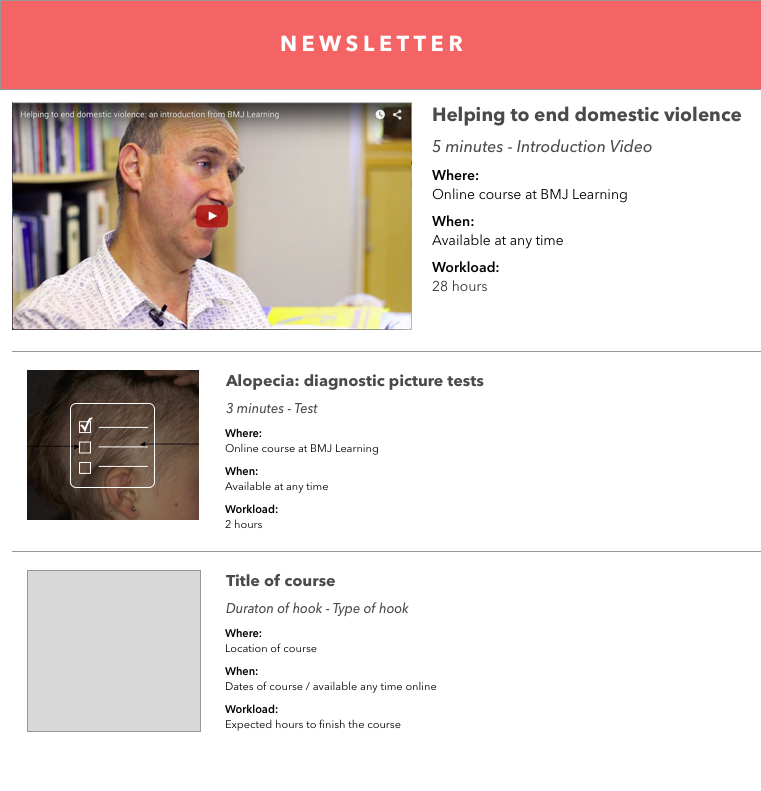
\includegraphics[width=1\textwidth]{figures/newsletter.png}
  \caption{Our mock-up of a newsletter simply presenting the course hooks.\label{fig:newsletter}}
 \end{center}
\end{figure*}

\section{Course page}
Figure \ref{fig:coursepage} shows our mock-up of how we envision the course page on the new DMA website should look, each such page presenting a course hook with additional information such as participant reviews, related courses and what else might be useful:

\begin{figure*}[h!]
 \begin{center}
  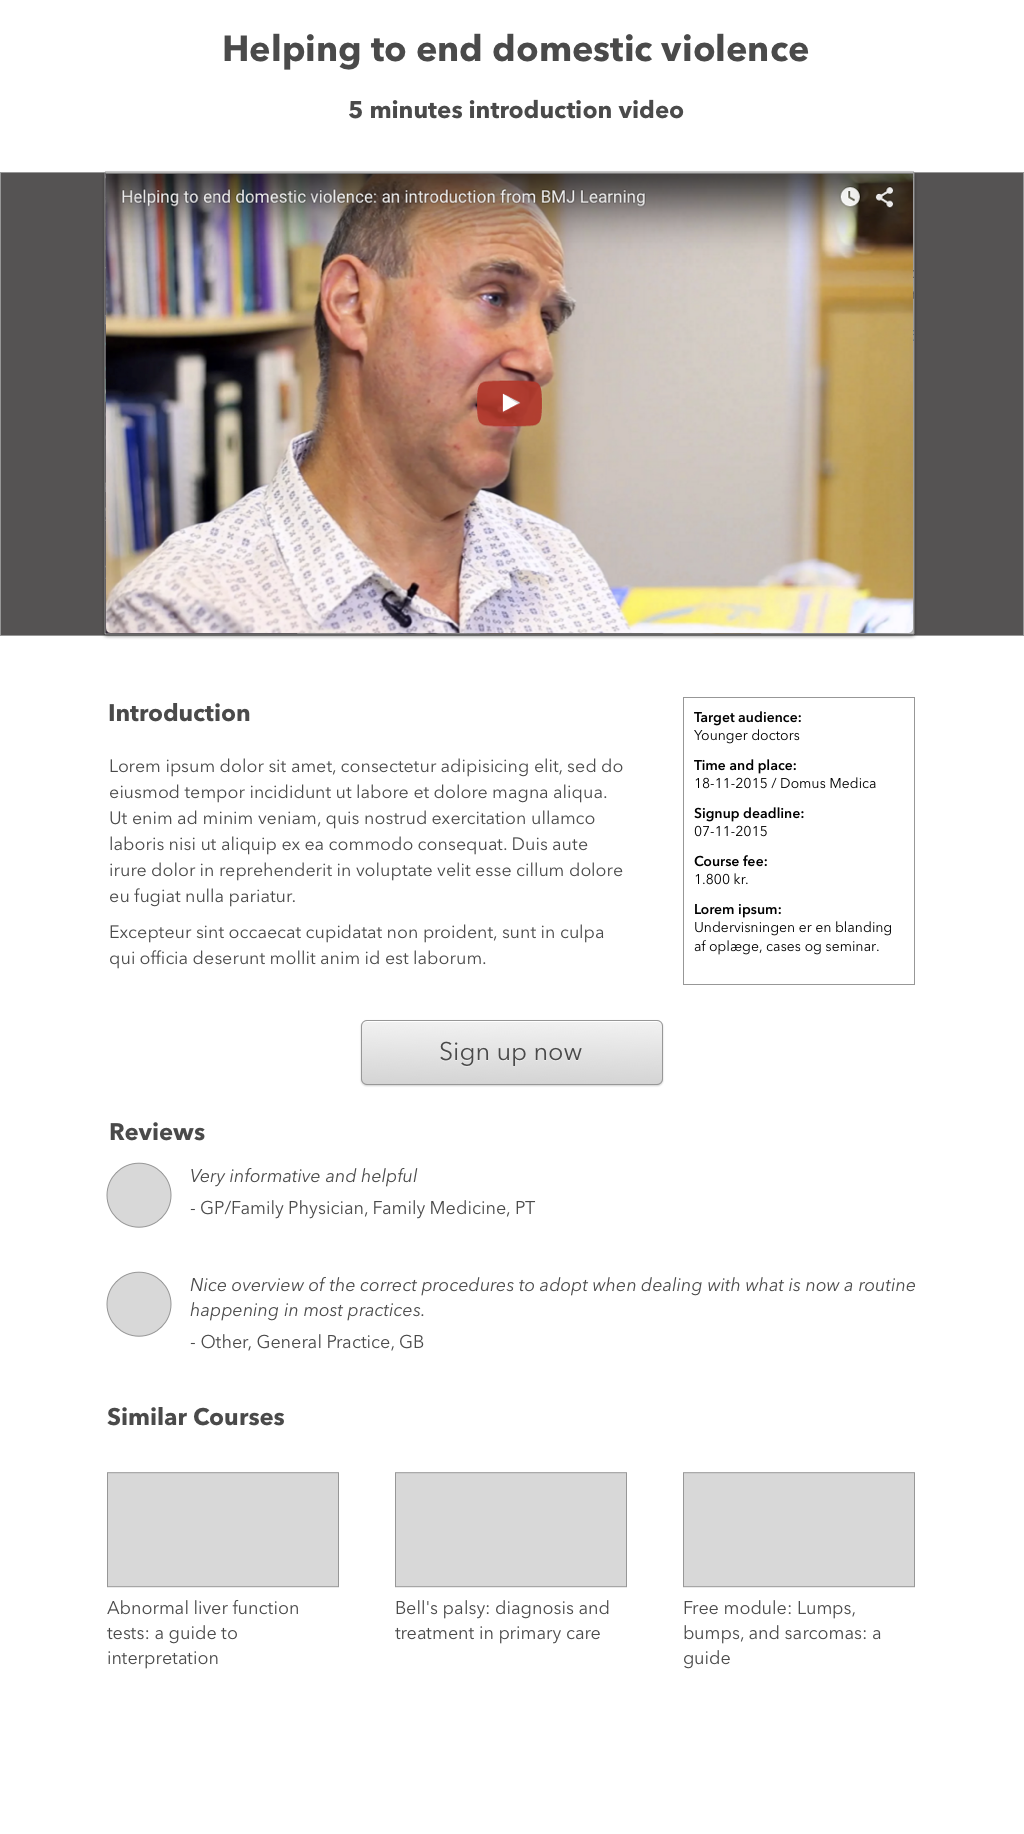
\includegraphics[width=1\textwidth]{figures/coursepage.png}
  \caption{Our mock-up of a course page presenting the course hooks.\label{fig:coursepage}}
 \end{center}
\end{figure*}

\end{appendices}
